\begin{frame}{Kalman Filter Overview}
\begin{center}
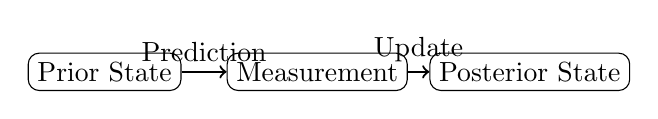
\begin{tikzpicture}[scale=0.9]
\node[draw, rounded corners] (prior) at (0,0) {Prior State};
\node[draw, rounded corners] (measurement) at (3,0) {Measurement};
\node[draw, rounded corners] (posterior) at (6,0) {Posterior State};

\draw[->, thick] (prior) -- node[above] {Prediction} (measurement);
\draw[->, thick] (measurement) -- node[above] {Update} (posterior);
\end{tikzpicture}
\end{center}
\vspace{0.5cm}
\begin{itemize}
\item Recursive state estimation algorithm
\item Optimal for linear systems with Gaussian noise
\item Maintains state estimate and uncertainty
\end{itemize}
\end{frame}

\begin{frame}{Kalman Filter Steps}
\begin{columns}[T]
\begin{column}{0.48\textwidth}
\textbf{Prediction Step}
\begin{center}
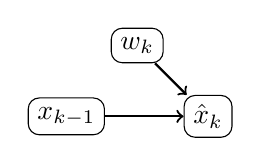
\begin{tikzpicture}[scale=0.9]
\node[draw, rounded corners] (state) at (0,0) {$x_{k-1}$};
\node[draw, rounded corners] (predicted) at (2,0) {$\hat{x}_k$};
\node[draw, rounded corners] (noise) at (1,1) {$w_k$};

\draw[->, thick] (state) -- (predicted);
\draw[->, thick] (noise) -- (predicted);
\end{tikzpicture}
\end{center}
\vspace{0.3cm}
\begin{align*}
\hat{x}_k &= F_k x_{k-1} + B_k u_k \\
P_k &= F_k P_{k-1} F_k^T + Q_k
\end{align*}
\end{column}

\begin{column}{0.48\textwidth}
\textbf{Update Step}
\begin{center}
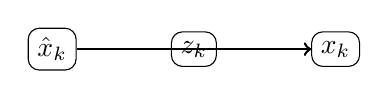
\begin{tikzpicture}[scale=0.9]
\node[draw, rounded corners] (pred) at (0,0) {$\hat{x}_k$};
\node[draw, rounded corners] (meas) at (2,0) {$z_k$};
\node[draw, rounded corners] (updated) at (4,0) {$x_k$};

\draw[->, thick] (pred) -- (updated);
\draw[->, thick] (meas) -- (updated);
\end{tikzpicture}
\end{center}
\vspace{0.3cm}
\begin{align*}
K_k &= P_k H_k^T (H_k P_k H_k^T + R_k)^{-1} \\
x_k &= \hat{x}_k + K_k(z_k - H_k \hat{x}_k) \\
P_k &= (I - K_k H_k)P_k
\end{align*}
\end{column}
\end{columns}
\end{frame}

\begin{frame}{Particle Filter Overview}
\begin{center}
\begin{tikzpicture}[scale=0.9]
\node[draw, rounded corners] (init) at (0,0) {Initial Particles};
\node[draw, rounded corners] (predict) at (3,0) {Prediction};
\node[draw, rounded corners] (update) at (6,0) {Weight Update};
\node[draw, rounded corners] (resample) at (9,0) {Resampling};

\draw[->, thick] (init) -- (predict);
\draw[->, thick] (predict) -- (update);
\draw[->, thick] (update) -- (resample);
\draw[->, thick] (resample) to[bend below] (predict);
\end{tikzpicture}
\end{center}
\vspace{0.5cm}
\begin{itemize}
\item Non-parametric approach to state estimation
\item Handles non-linear systems and non-Gaussian noise
\item Represents state distribution with weighted particles
\end{itemize}
\end{frame} 